%# -*- coding: utf-8-unix -*-
%%==================================================
%% chapter01.tex for SJTU Master Thesis
%%==================================================

%\bibliographystyle{sjtu2}%[此处用于每章都生产参考文献]
\chapter{绪论}
\label{chap:intro}

大数据时代的到来和云计算的迅猛发展使得用分布式计算的方式来处理海量数据的方案变得水到渠成。
分布式并行计算框架的出现,特别是基于有向无环图(DAG)的方式来表达计算逻辑的分布式计算框架,进一步简化了大数据处理的过程。
也正是如此,使得分布式计算框架在短时间内获得了大量的普及。
虽然如何使得分布式计算变得更高效一直是近几年的研究热点,但是大量工作都集中在优化计算阶段的方向。
而对于其中shuffle阶段则关注较少。但是不能忽视的是,在许多场景下,shuffle这种I/O密集型的操作甚至会成为整个分布式计算应用的性能瓶颈。
本文针对现有的基于DAG的分布式计算框架的shuffle特点,提出了一种通用,高效的shuffle优化方案。
本文首先会介绍基于DAG分布式计算框架以及其优化的研究背景,然后阐述本文的优化目标以及国内外相关研究现状,最后简单介绍本文的结构组成。

\section{研究背景}

大数据时代的到来使得企业要处理的数据量远远超过了一台机器的处理性能。
在分布式计算普及之前,企业只能通过不断升级昂贵的超级计算机的性能来满足指数级增长的数据量。
然而随着Google公开了MapReduce\cite{mapreduce}的并行计算模式之后,分布式并行计算逐渐进入了蓬勃发展的阶段。
相对于昂贵而复杂的大型机,分布式计算能使用造价较低的商用机,并通过网络组合成集群,从而提供与超级计算机相匹配的运算能力来对大数据进行批处理。
最近几年,更是有大量的分布式计算框架在学术界和工业界得以发表和公开同时也有大量的计算框架被部署到企业的生产环境中,成为大数据生态系统中最重要的一个组件。
其中应用最广泛的就是Hadoop MapReduce\cite{mapreduce},Spark\cite{apachespark}和Tez\cite{tez}等。

\begin{figure}[!htp]
	\centering
	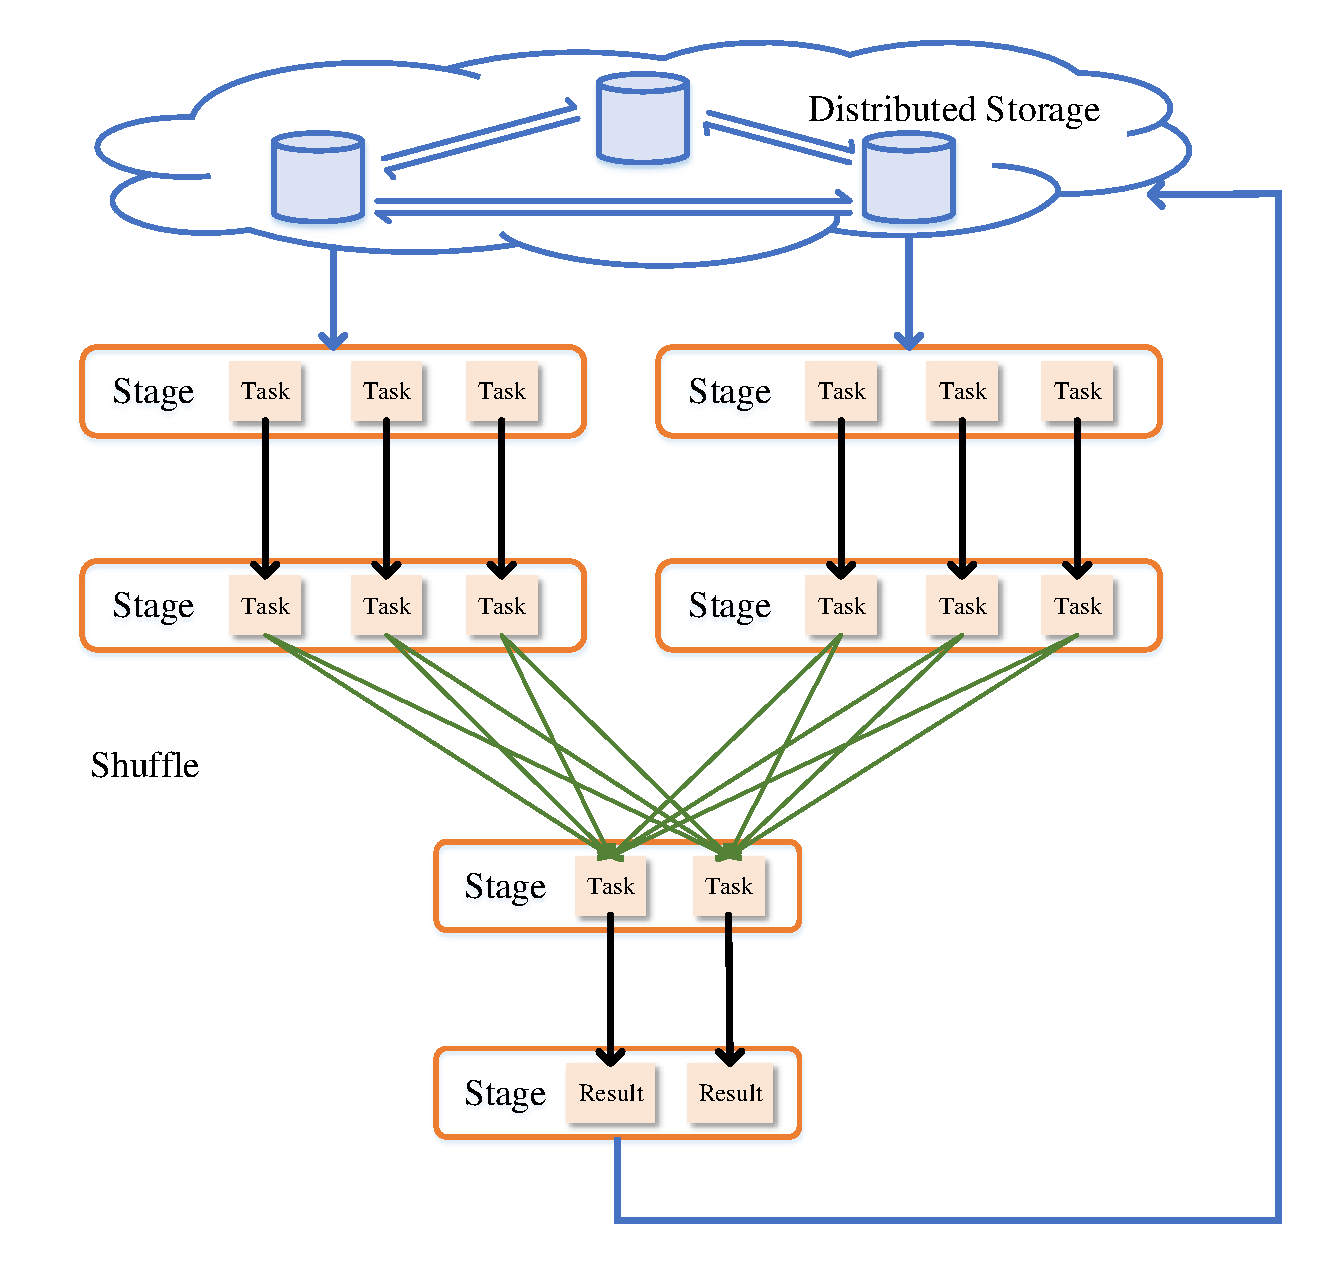
\includegraphics[width=\textwidth]{dagOverview.pdf}
	\bicaption[fig:dagOverview]{分布式DAG计算框架执行示意图}{分布式DAG计算框架执行示意图}{Fig}{Overview of DAG computing frameworks}
\end{figure}

如图\ref{fig:dagOverview}所示,这些计算框架通过有向无环图(DAG)的方式来表达用户应用逻辑。
在执行DAG的过程中,对于每一个计算阶段(stage)采用了整体同步并行计算模型(BSP)来对大数据进行分布式的并行批处理。
在一个计算阶段,框架会将数据分块,并且对于每一块数据应用相同的用户定义计算来进行并行处理,既图\ref{fig:dagOverview}中的task。
在DAG的执行过程中,每一个任务都会有对上一个任务的数据依赖。这个数据依赖可以被分成两个类型:完全依赖和部分依赖。
完全依赖指的是当前计算阶段的一个任务所需要的输入数据完全依赖于上一个计算阶段的一个或几个任务的所有输出数据,比如图\ref{fig:dagOverview}中黑色箭头所表示的依赖关系。
部分依赖,也就是本文中提到的shuffle,则表示当前计算阶段的一个任务所需要的输入数据依赖于上一个计算阶段的多个任务的部分数据,比如图\ref{fig:dagOverview}中绿色的部分。
通常而言,对于产生shuffle数据的一端,我们称之为映射阶段(Map Stage),而对于接收shuffle数据的一端,我们称之为规约阶段(Reduce Stage)。
对于完全依赖,目前已经有了好的解决方案。比如Spark\ref{apachespark}中RDD\ref{spark}的解决方案,就通过将连续的完全依赖的计算阶段合并成一个大的计算阶段,并且通过内存计算的加速来优化了这部分数据依赖。

但是对于shuffle的依赖,虽然这些DAG计算框架在设计上存在很多不同,但是他们都是通过多对多的网络数据传输方式来实现。
而shuffle阶段由于受限于I/O设备性能的限制(磁盘,网络等),会对整个端到端的应用执行性能带来很大的额外开销。
虽然近几年针对分布式DAG计算框架的计算阶段学术界和企业界都提出了很多优化方案\cite{pacman, babu, quincy, sync},但是对于shuffle阶段在实际应用中的优化却一直很不理想。
比如在Facebook公开的一个MapReduce运行数据分析中,shuffle平均占到了所有任务完成时间的33\%。
对于需要大量shuffle的一些任务,shuffle的开销最多可以占到整个任务完成时间的70\%\cite{managing}。

\section{研究内容}

本文通过对这些计算框架的研究,发现制约shuffle性能的主要是由于缺乏对于不同类型的硬件资源的细粒度的管理和调度。
在目前的DAG计算框架调度算法中,对于一个计算阶段的每一个任务,DAG计算框架的调度器都会分配集群中一部分固定的硬件资源,包括CPU,内存,磁盘和网络等。
为了简化调度算法,这些资源被捆绑成一个slot来进行粗粒度的管理和分配。
这种粗粒度的调度算法虽然简化了调度过程,但是也引入无法充分利用硬件资源的问题。
比如,当一个任务进行CPU内存密集的数据计算时,该slot所占用的I/O资源就会被限制。反之,当任务进行I/O密集的shuffle过程时,CPU和内存等计算资源就会被闲置。

除此之外,在shuffle阶段不可避免得会引入多对多的网络数据传输。
在目前的分布式DAG计算框架中,此阶段的网络数据传输也没有得到很好的管理。
当reduce阶段被调度并启动之后,集群中会有多个reduce任务同时启动,并且几乎同时通过网络来从远程节点获取数据。
这种几乎同步的数据传输模式会给集群的网络带来一个瞬时的流量高峰。
而当带宽有限的情况下,这种瞬时的高峰极易造成网络的拥塞,从而进一步减慢了数据传输的速率。

更糟糕的是,上述发现的问题存在于大部分主流的分布式DAG计算框架当中。所以仅仅只是针对其中某一个框架提出解决方案并不能很好的缓解shuffle给分布式计算带来的性能开销。

为了给shuffle过程提供一个具有普适性的优化方案,本文提出了S(huffle)Cache --- 一个开源的即插型shuffle管理系统来给不同的DAG计算框架提供高效的shuffle管理和优化。
具体来说,SCache通过提供跨框架的API设计,来接管在DAG计算过程中的shuffle阶段。
同时SCache采用了以下几点关键创新,来实现对于shuffle的高效管理和优化:

\begin{enumerate}
	\item 将shuffle从计算过程中的解耦。使得shuffle的过程独立到DAG计算框架外部进行管理,从而实现了更细粒度的硬件资源管理,提高硬件资源的复用率和利用率,进而加速shuffle过程。
	\item 结合应用的上下文对reduce任务进行预调度。采取了启发式算法,根据map阶段执行过程中的中间状态,结合应用的上下文逻辑和数据本地性等特征提前调度reduce阶段的任务。
	\item 对shuffle数据进行预取。在map执行阶段,根据启发式预调度算法的结果,对shuffle数据进行预取,既避免了同步数据读取给网络带来的压力,又能将大部分网络传输时间隐藏到计算的阶段。
	\item 采用了结合上下文的内存管理机制。根据DAG计算框架的任务调度策略,对不同的shuffle数据块设置优先级,同时提前将shuffle数据缓存在内存当中,加速shuffle数据的读取过程,提升任务计算性能。
	\item 设计了具有普适性的API。SCache不仅根据shuffle的读写为DAG计算框架设计了相应的API,同时也为DAG框架的调度器设计了相应提交shuffle相关元数据和获取预调度结果的API。
\end{enumerate}

\section{国内外研究现状}
\label{sec:relatedwork}

目前国内外的对shuffle的优化工作主要分成三个方向:提前调度,延迟调度和纯网络层面的优化。

\textbf{提前调度}:Slow-start作为Hadoop MapReduce\cite{hadoop}中最经典的shuffle优化是提前调度的代表性方案。
Starfish\cite{starfish}通过对数据的采样来自动调整MapReduce中的系统参数,比如slow-start的比例,map和reduce任务的比例等待。
DynMR\cite{dynmr}通过动态的在map阶段末端启动reduce任务来减少对与shuffle数据的等待。
以上所有这些方案都没有将I/O操作从计算密集型的任务中解耦,因而仍然在slot中留下显示的I/O等待时间。
而且由于计算资源有限,提前启动reduce任务会占用有限的slot,减慢map阶段的执行。
所以在设定何时启动提前调度的参数时,会受到应用,输入数据,当前硬件资源等条件的影响,不仅参数设置困难,优化效果也会有较大波动。
iShuffle\cite{ishuffle}采用了讲shuffle从reduce阶段解耦的方式,并且提供了一个中心控制器来调度shuffle。但是这个方案并不能和好的处理对多个shuffle的依赖。
iHadoop\cite{ihadoop}采用了激进地提前调度多个接下来的计算阶段的任务,从而是的shuffle数据的预取成为可能。
Drizzle\cite{drizzle}也采用了提前调度任务的方式来实现shuffle数据的预取。
但是在我们研究过程中发现,随机激进地调度任务可能会破坏DAG计算框架的负载均衡,从而减慢应用的性能。

\textbf{延迟调度}:Delay Scheduling\cite{delay}采用延迟分配任务来获取更好的数据本地性,进而减少了shuffle阶段的网络数据传输。
ShuffleWatcher\cite{shufflewatcher}会在网络将近饱和的时候延迟shuffle数据的获取。同时它能在调度任务时获取更好的本地行。
Quincy\cite{quincy}和Fair Scheduling\cite{preemptive}都可以通过优化map任务的调度来获取更好的shuffle数据本地性。
但是以上这些工作都不能消除在计算任务中显示的I/O操作。更重要的是,他们的优化效果会因为网络的性能好坏和计算数据的不同分布而产生波动。

\textbf{网络层优化}:Varys\cite{varys},Aalo\cite{aalo},CODA\cite{coda},Seagull\cite{seagull}都能结合应用层信息提供shuffle在网络传输时的优化,从而加快shuffle的传输过程。
而DCTCP\cite{dctcp},pFabric\cite{pfabric},Pias\cite{pias},CONGA\cite{conga}等工作能结合数据中心网络的特点在纯网络层降低网络流的平均完成时间,增加网络吞吐。
虽然这些优化仅仅局限在shuffle过程中的网络传输部分,但是它们可以为本研究的优化提供进一步的性能提升。

\section{文章结构}

本文余下内容结构如下:

第二章介绍shuffle在分布式并行DAG计算框架中的特点以及相关背景。通过对shuffle特性的分析,来挖掘其可优化的空间和制定具体优化方案。

第三章详细介绍了SCache的具体设计与实现,包括SCache的架构,shuffle调度算法设计,接口设计以及内存管理策略。
同时还会介绍SCache和Spark协同工作的实例。

第四章对SCache在Spark平台上的优化效果进行了实验和分析。
通过仿真实验和Amazon AWS EC2上虚拟机集群的测试,验证了SCache在shuffle上的优化效果。

第五章对全文进行了总结,并且对未来的工作方向做出展望。







